\documentclass[a4paper, 10pt]{article}
\usepackage[T1]{fontenc}
\usepackage[utf8]{inputenc}
\usepackage[slovene]{babel}
\usepackage{csquotes}
\usepackage{lmodern}
\usepackage{amsmath}
\usepackage{leftidx}
%\usepackage[backend=biber, style=numeric]{biblatex}
\usepackage{amssymb}
\usepackage{amsthm}
\usepackage{amsfonts}
\usepackage{graphicx}
\usepackage{wrapfig}
\usepackage{amsthm}
\usepackage{mathrsfs}
\usepackage{mathtools}
\usepackage{url}
\usepackage{subfigure}
\usepackage{multirow}
\usepackage{lipsum}
\usepackage{wrapfig}
\usepackage{tikz}
\usepackage[format=plain, font=small, labelfont=bf, textfont=it, justification=centerlast]{caption}
\usepackage{booktabs}
\usepackage{siunitx}
%\usepackage{cleveref}

\newtheorem{izr}{Izrek}
\newtheorem*{izr*}{Izrek}
\newtheorem{lem}{Lema}
\newtheorem{trd}{Trditev}
\newtheorem*{trd*}{Trditev}
\newtheorem{posl}{Posledica}[izr]

\newcounter{defcount}
\newcounter{opombe}
\newcounter{primercount}
\newcounter{zgledcount}

\newenvironment{opomba}{\begin{flushleft}\refstepcounter{opombe}\textbf{Opomba \arabic{opombe}:}}{\hfill\end{flushleft}}
\setlength{\parindent}{0mm}

\newenvironment{primer}{\begin{flushleft}\refstepcounter{primercount}\textbf{Primer \arabic{primercount}:}}{\hfill\end{flushleft}}
\setlength{\parindent}{0mm}

\newenvironment{zgled}{\begin{flushleft}\refstepcounter{zgledcount}\textbf{Zgled \arabic{zgledcount}:}}{\hfill\end{flushleft}}
\setlength{\parindent}{0mm}

\newenvironment{definicija}{\begin{flushleft}\refstepcounter{defcount}\textbf{Definicija \arabic{defcount}:}}{\hfill\end{flushleft}}
\setlength{\parindent}{0mm}

\newcommand{\naslov}[1]{\textit{#1}}
\newcommand{\abs}[1]{\ensuremath{\lvert #1 \rvert}}
\newcommand{\mth}[1]{\ensuremath{\mathbb{#1}}}
\newcommand{\R}{\mth{R}}
\newcommand{\Z}{\mth{Z}}
\newcommand{\Zp}{\mth{Z}^{+}}
\newcommand{\N}{\mth{N}}
\newcommand{\No}{\mth{N}_0}
\newcommand{\C}{\mth{C}}
\newcommand{\Q}{\mth{Q}}
\newcommand{\Qu}{\mth{Q}_u}
\newcommand{\pojem}[1]{\emph{#1}}
\newcommand{\con}{\ensuremath{\mathscr{C}}}
\newcommand{\padex}[2]{\ensuremath{{#1}^{\underline{#2}}}}
\newcommand{\rastx}[2]{\ensuremath{{#1}^{\bar{#2}}}}
\newcommand{\map}[3]{\ensuremath{{#1}: {#2} \rightarrow {#3}}}
\newcommand{\pra}[3]{{#1}{\ast}({#2}) = {#3}}

\title{Arhimed, O ravnovesju ravnin\\ {\large Seminarska naloga pri predmetu Zgodovina matematike}}
\date{30.~12.~2024}
\author{Jimmy Zakeršnik}
%===============================================================================
\begin{document}
	\maketitle
	\thispagestyle{empty}
	\newpage
	%\tableofcontents
	\newpage
	\section{Uvod}
		Arhimed spada med najpomembnejše matematike evropske Antike, predvsem zaradi svojih dosežkov na področjih geometrije in mehanike. V svojem delu ">O ravnovesju ravnin"< v dveh knjigah na povsem geometrijski način obravnava težišča raznih ravninskih likov in njihove lastnosti. V prvi knjigi določi težišča poljubnega trikotnika, paralelograma in trapeza, celotna druga knjiga pa je posvečena določanju težišča poljubnega paraboličnega odseka. V nadaljevanju bodo bolj podrobno predstavljeni njegovi rezultati. Pri tem bodo podatki črpani predvsem iz \cite{bib:Heath}.
	\section{Prva knjiga}
		Arhimed prvo knjigo prične s sedmimi postulati, ki nam (v povzeti obliki) povedo naslednje: \begin{enumerate}
			\item Enako oddaljeni teži sta v ravnovesju.
			\item Če, ko sta teži na dani razdalji v ravnovesju, eno od njiju povečamo ali zmanjšamo, teži več nista v ravnovesju, temveč se nagneta proti tisti, ki se je povečala oz. se ni zmanjšala.
			\item Če ravninska lika, ko nesemo enega na drugega, sovpadata, potem sovpadata tudi njuni težišči.
			\item Če sta si neskladna lika podobna, sta tudi njuni težišči ">postavljeni podobno"<. 
			\item Težišče vsakega lika, katerega rob je konkaven v natanko eni smeri, se nahaja znotraj lika.
		\end{enumerate}
		
		Iz omenjenih postulatov s pomočjo dokaza s protislovjem Arhimed nato dokaže pet preprostih trditev, nato pa še t.i. ">zakon o vzvodu"<:\begin{izr*}[Zakon o vzvodu]
			Veličini sta v ravnovesju na razdaljah, ki sta obratno sorazmerni z veličinama.
		\end{izr*} 
		Rezultat najprej direktno dokaže za somerljive like v trditvi $VI$, nato pa še za nesomerljive like v trditvi $VII$ s pomočjo dokaza s protislovjem. V trditvi $VIII$ Arhimed poda metodo, kako se določi težišče nekega dela veličine, če imamo podano težišče preostanka in težišče celotne veličine. V trditvah $IX$ in $X$ Arhimed določi težišče poljubnega paralelograma takole: 
		\begin{trd*}[Trditev $IX$]
			Težišče poljubnega paralelograma leži na daljici, ki povezuje središči nasprotnih stranic.
		\end{trd*}
		\begin{proof}
			Naj bo $ABCD$ poljuben paralelogram in označimo z $E$ razpolovišče stranice $AD$ ter z $F$ razpolovišče $BC$. Označimo s $H$ težišče paralelograma. Denimo, da se $H$ ne nahaja na daljici $EF$. Tedaj s $K$ označimo presečišče daljice $EF$ in vzporedinice stranici $BC$ skozi $H$. Sedaj razpolovimo daljici $AE$ in $ED$, nato razpolovimo dobljene polovice in postopek nadaljujemo, dokler ne dobimo kosov, ki so krajši od $HK$. Sedaj skozi vsako delilno točko potegnemo vzporednico s stranico $AB$ ter tako naš paralelogram razrežemo na več manjših medseboj skladnih paralelogramov, kot na sliki.
			\begin{figure}[h!]
				\centering
				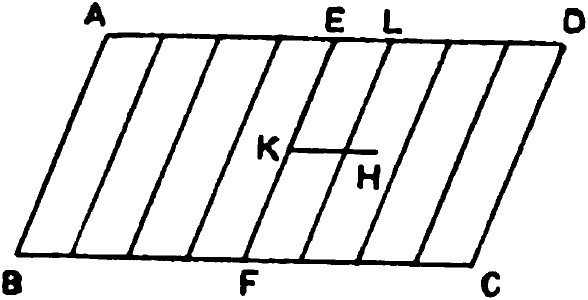
\includegraphics[scale=0.5]{Paralelogram.jpg}
				\caption{Slika paralelograma iz dokaza}
			\end{figure}
			Ker so paralelogrami medseboj skladni, so si medseboj podobni, torej bodo tudi njihova težišča ">podobno postavljena"<. Pred seboj imamo torej končno mnogo enako velikih veličin, katerih težišča so po neki daljici porazdeljena ekvidistančno. Posledično se težišče celote (paralelograma $ABCD$) nahaja na daljici, ki povezuje težišči srednjih dveh manjših paralelogramov (tistih dveh, ki imata $EF$ za eno od stranic). Tukaj pa pridemo v protislovje, saj se težišče paralelograma $ABCD$, ki smo ga označili s $H$, ne nahaja znotraj omenjenih manjših paralelogramov. Sledi, da se težišče nujno nahaja na $EF$.
		\end{proof}
		Nadaljno v trditvah $XIII$ in $XIV$ določi težišče poljubnega trikotnika, v trditvi $XV$ pa določi težišče poljubnega trapeza. 
	\section{Druga knjiga}
		V drugi knjigi Arhimed obravnava težišča paraboličnih odsekov ter delov paraboličnih odsekov, ki se nahajajo med osnovnico in neko njeno dano vzporednico.
		Najprej v trditvi $I$ pokaže, da če sta $P$ in $P'$ ploščini danih paraboličnih odsekov in $D$ ter $E$ njuni težišči, potem se težišče obeh likov skupaj nahaja v točki $C$ na daljici $DE$, za katero velja $$P:P' = CE:CD $$
		Podobno kot pri izračunu ploščine paraboličnega odseka, tudi tukaj Arhimed v odsek včrta lik na t.~i.~">znan način"<: V odsek najprej včrta trikotnik $\triangle AB'B$ z enako osnovnico in višino (označimo z $O$ stičišče osnovnice in višine tega trikotnika). Nato v odseka, ki sta omejena s stranicama trikotnika in pripadajočim odsekom ponovno včrta trikotnika na enak način - označimo dobljena vrha na paraboli z $Q$ in $Q'$. V odsekih, ki ju določajo stranice trikotnikov $\triangle ABQ$ in $\triangle AQ'B'$ postopek ponovimo in tako označimo še vrhove $P, P', R, R'$.
		
		Dodatno, v lemah pred trditvijo $II$ pokaže, da za včrtan lik $AP'Q'R'B'BRQP$ velja, da premeri parabole, ki tečejo skozi točke $Q, Q', P, P', R$ in $R'$ razpolovijo daljice $AB, AB', AQ, AQ', QB$ in $Q'B'$ ter hkrati razdelijo daljico $BB'$ na enake dele. Še več, Arhimed pokaže, da so daljice $PP', QQ'$ in $RR'$ vzporedne daljici $BB'$, ter da presečišča teh daljic z višino $AO$ paraboličnega odseka (označimo jih z $L, M, N$) razdelijo višino v razmerju $AL:LM:MN:NO = 1:3:5:7$, ter da enako velja, če bi povečali število stranic včrtanega lika - odseki daljice $AO$ so zmeraj v razmerju zaporednih lihih števil. 
		\begin{figure}[h!]
			\centering
			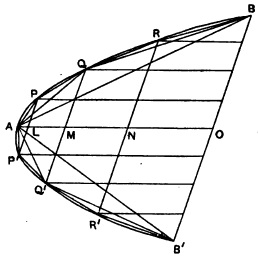
\includegraphics[scale=0.75]{Parabol.jpg}
			\caption{Slika paraboličnega odseka z včrtanim likom}
		\end{figure}
		
		V trditvi $II$ Arhimed dokaže, da težišče danega včrtanega lika leži na višini $AO$, v trditvi $IV$ pa tudi, da enako velja za pripadajoči parabolični odsek. Slednjo trditev dokaže s protislovjem, na podoben način kot za trikotnik v prvi knjigi. V trditvi $V$ Arhimed pokaže, da je težišče paraboličnega odseka bližje točki $A$, kot pa težišče včrtanega lika, v trditvi $VI$ pa pokaže, da lahko v parabolični odsek na znan način včrtamo lik tako, da je razdalja med težiščema manjša od poljubne dane razdalje. V trditvi $VII$ Arhimed dokaže, da težišči podobnih paraboličnih odsekov razdelita njuni višini v enakem razmerju. Ta rezultat sicer velja za poljubna dva parabolična odseka, kar je tudi potrebno pri Arhimedovem dokazu trditve $VIII$. V omenjeni trditvi $VIII$ Arhimed določi težišče poljubnega paraboličnega odseka s pomočjo predhodne trditve. Gre v resnici za geometrični način reševanja preproste enačbe $$\frac{1}{3}\cdot(1+m) + 4\cdot\frac{2}{3} = 4m\cdot\frac{4}{3}$$ v kateri je spremenljivka $m$ razmerje med $AG$ in $AO$, kjer je $G$ težišče paraboličnega odseka. Rešitev je seveda $m = \frac{3}{5}$, torej je težišče paraboličnega odseka tista točka $G$ na premeru $AO$, da je $AG:GO = 3:2$.
	
		V zadnji trditvi, trditvi $X$, Arhimed določi težišče kosa paraboličnega odseka, ki je omejen z osnovnico in neko njeno vzporednico. Denimo, da je dani kos omejen z osnovnico $BB'$ in njej vzporedno ter krajšo daljico $PP'$. Z $N$ in $O$ označimo razpolovišči $PP'$ in $BB'$. Sedaj $NO$ radelimo na pet enakih delov in sredinskega označimo z $LM$ (kjer je $L$ bližji $N$). Tedaj je težišče tega dela parabole med $PP'$ in $BB'$ točka $G$ na daljici $LM$, za katero velja:
		$$LG:GM = BO^2\cdot(2PN + BO):PN^2\cdot(2BO + PN)$$
		Arhimedov dokaz, ki je povsem geometričen, je precej zahteven in sloni na uporabi trditve $IX$: Naj bodo $a, b, c, d, x$ in $y$ daljice; kjer so $a>b>c>d$; za katere veljajo naslednji pogoji: \begin{itemize}
		\item $a:b = b:c = c:d$
		\item $d:(a-d) = x: \frac{3}{5}(a-c)$
		\item $(2a+4b+6c+3d) : (5a+10b+10c+5d) = y: (a-c)$
		\end{itemize}
		Tedaj je $x + y = \frac{2}{5}a$.

	\begin{thebibliography}{99}
		
		\bibitem{bib:Heath} T.~Heath,~\emph{A history of Greek mathematics volume $2$}, Dover Publications, New York, 1981.
		
	\end{thebibliography}
\end{document}